\documentclass{article}

\usepackage[letterpaper, portrait, margin=1.5in]{geometry}

\usepackage{fancyhdr}
\usepackage{ragged2e}
\usepackage{graphicx}
\usepackage{caption}
\usepackage{amsmath}
\usepackage{rotating}

\usepackage{listings}
\usepackage{color}

\definecolor{dkgreen}{rgb}{0,0.6,0}
\definecolor{gray}{rgb}{0.5,0.5,0.5}
\definecolor{mauve}{rgb}{0.58,0,0.82}

\lstset{frame=tb,
  language=Java,
  aboveskip=3mm,
  belowskip=3mm,
  showstringspaces=false,
  columns=flexible,
  basicstyle={\small\ttfamily},
  numbers=none,
  numberstyle=\tiny\color{gray},
  keywordstyle=\color{blue},
  commentstyle=\color{dkgreen},
  stringstyle=\color{mauve},
  breaklines=true,
  breakatwhitespace=true,
  tabsize=4
}

\setcounter{secnumdepth}{1}

\usepackage{chngcntr}
\counterwithin{figure}{section}

\renewcommand*{\thepage}{C\arabic{page}}

\pagestyle{fancy}
\lhead{ACME Robotics}
\chead{\#8367}
\rhead{\ifcontents Contents \else Week \thesection \fi}

\newif\ifcontents
\contentstrue

\makeatletter
\renewcommand{\@seccntformat}[1]{}
\makeatother
\begin{document}
\subsection{Cartridge Servo}
%! Decreasing the load on the cartridge servo.
While Aidan and Kelly were testing the subsystems they saw that the cartridge servo was having trouble doing its full rotation. The servo especially had a problem when there was two cubes in the diverter because that is when it was carrying the most weight. The servo seemed to have trouble with the up part of its dump rotation as well as the up part of its reverse rotation. This caused a problem because it meant that whatever was used to help the servo needed to help it in both directions. Kelly and Aidan solved this by attaching a quadrupled up piece of surgical tubing to a stationary piece of the carriage and the other side to the servo horn. They connected it so that when the carriage was at its balancing point the surgical tubing had the least amount of tension. They did this so that when rotated farther clockwise then its balancing point the surgical tubing would help the servo in its reverse rotation and when rotated farther counterclockwise then its balancing point the tubing would help in the dump rotation. This helped the servo and allowed it to rotate in both directions with little difficulty.

\begin{figure}
    \centering
    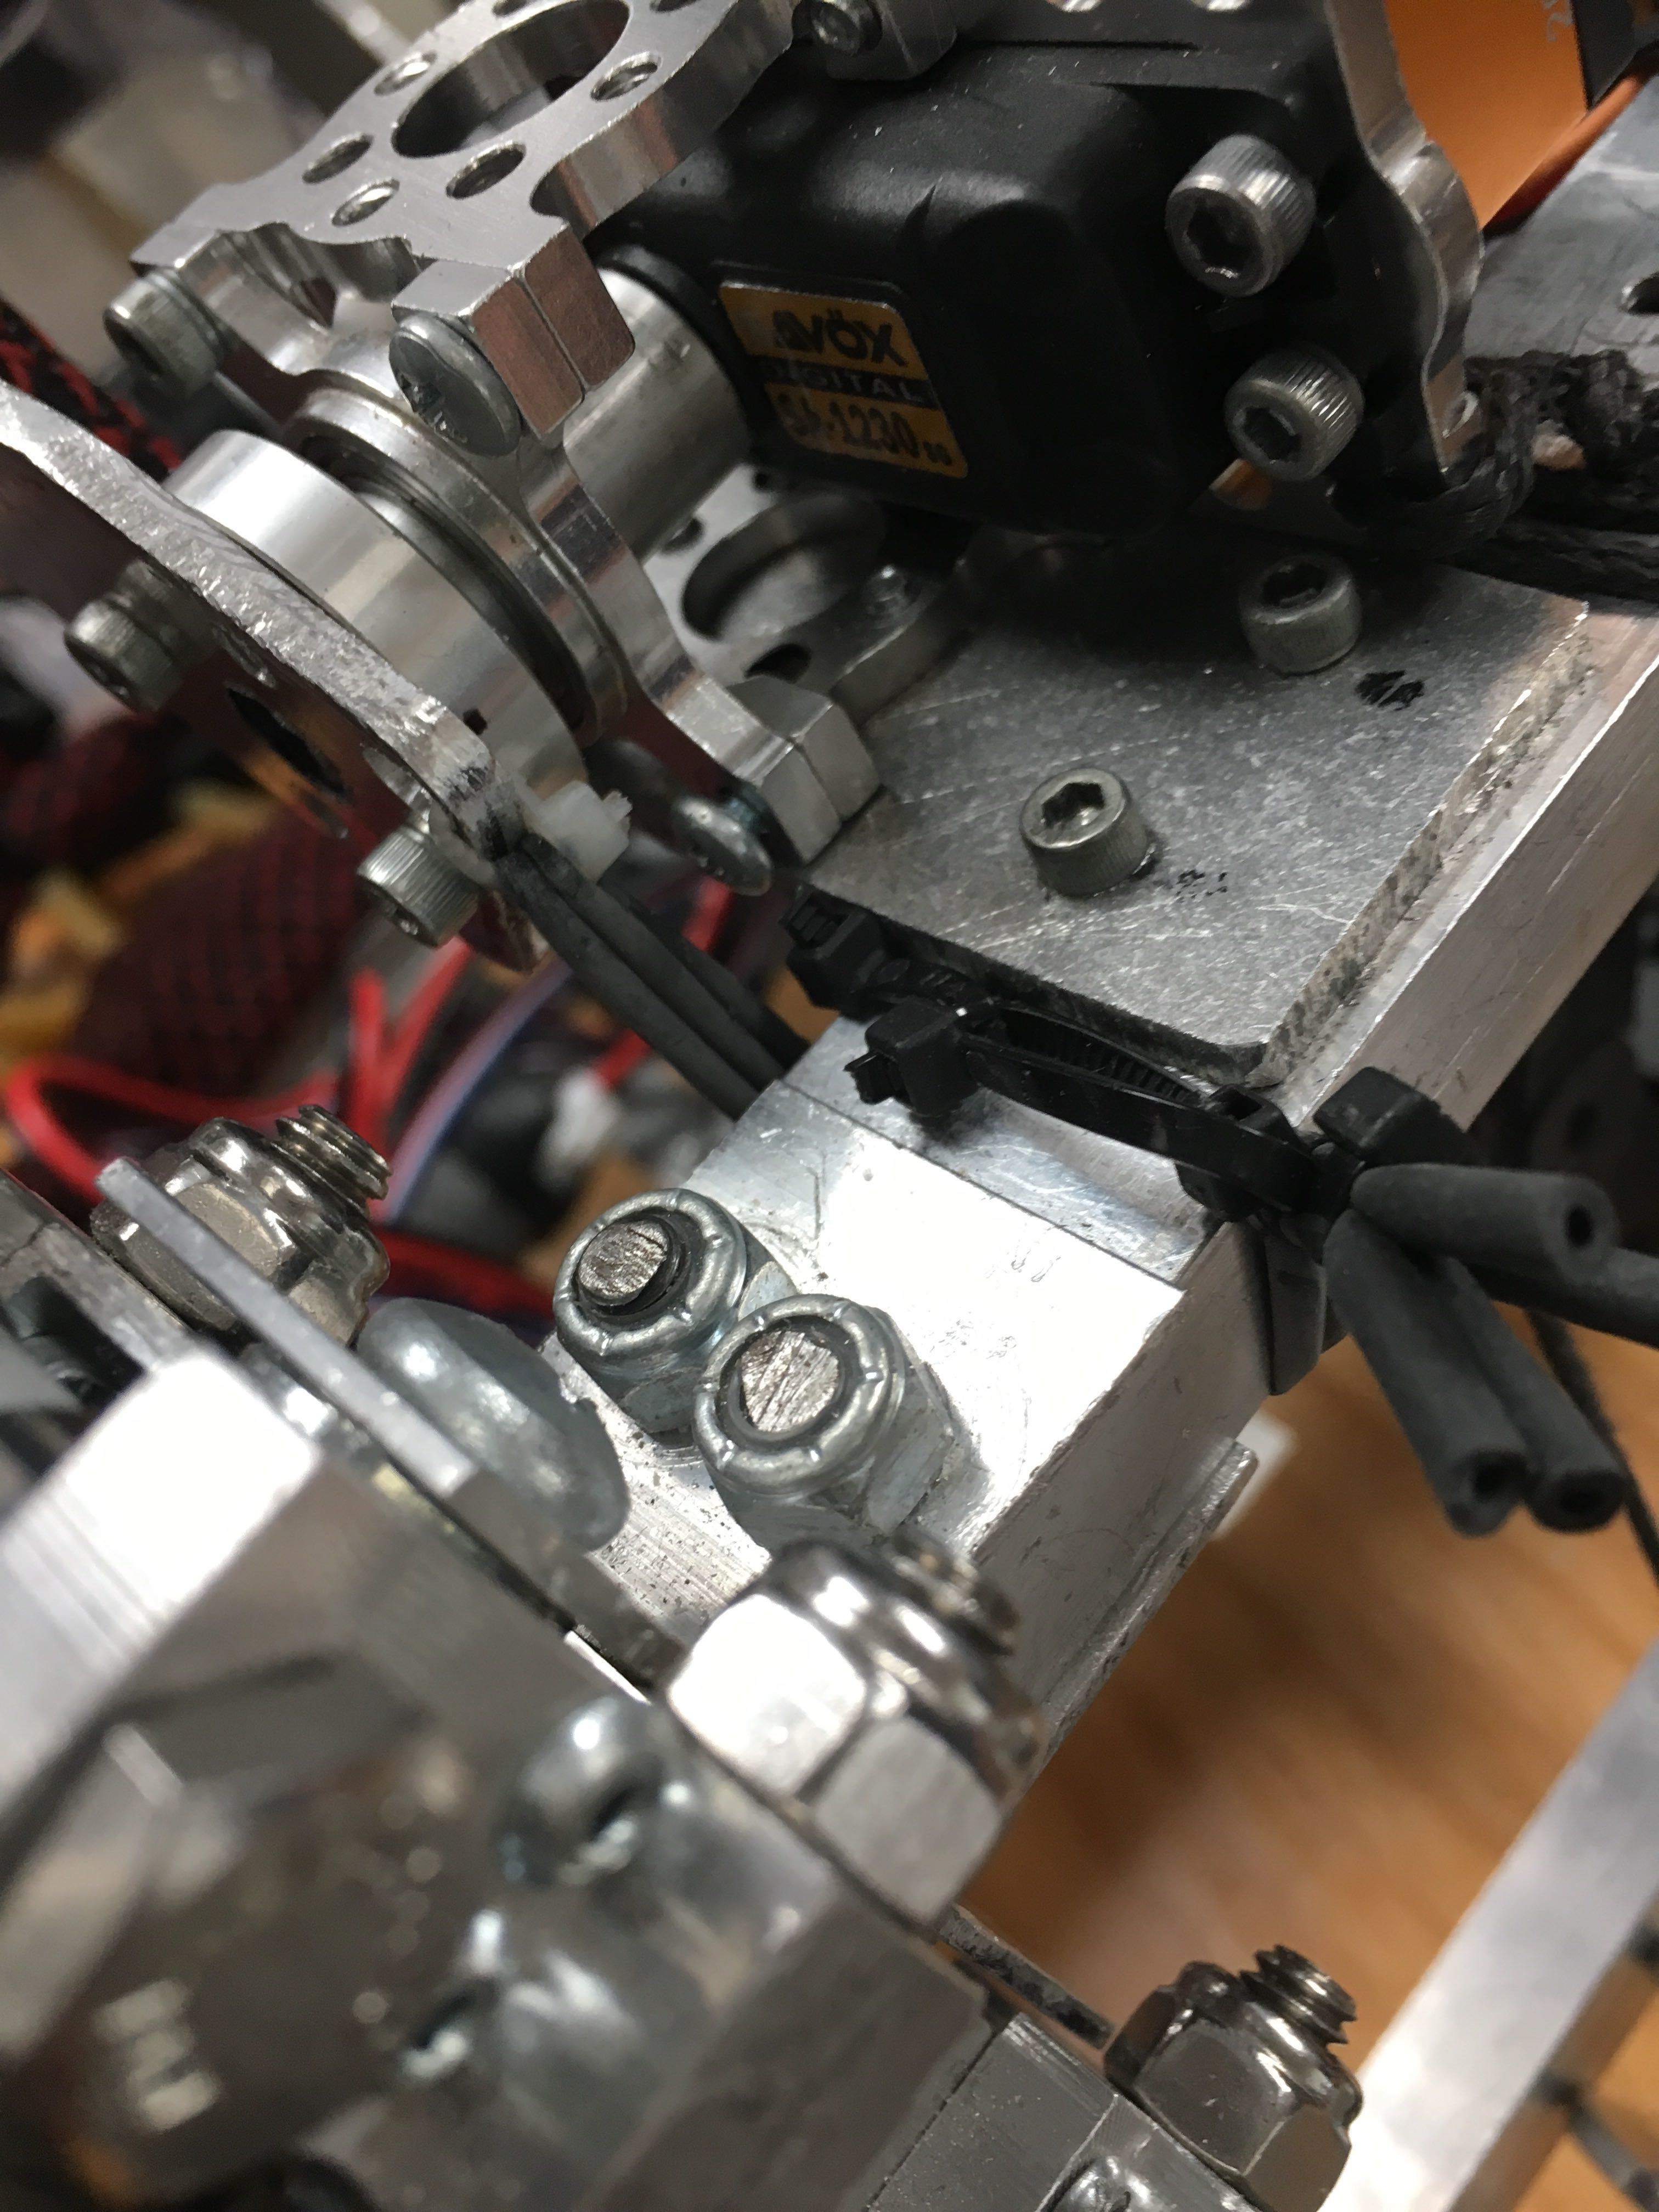
\includegraphics[width=.6 \textwidth]{21_01-21/images/tubing.JPG}
    \caption{Surgical Tubing}
    \label{fig:tubing}
\end{figure}

\subsection{Lift Skids}
%! Brainstorm ideas for the lift skids.
With the lift now in working order, the team conducted some tests with it to see if it was up to snuff. The team quickly found that the lift didn't quite have the robot hanging the full four inches off the floor. The team put Aidan, Ashlin, and Jon on the job to fix this issue. They found that the robot was angled in such a way that the front was lower than the back. This meant that even though the back of the robot was four inches off the ground, the front was not. This was because the top of the lift stuck out farther (because of the hook) than the bottom. The trio thought they could add a plate to the back of the robot to alleviate this problem. They thought if they put a plate that stuck out as far as the hook, the robot would be flush with the lander along the entire robot. This would also make sure none of the lift or back of the robot would get caught on the lander and would just overall smooth the lifting and lowering process. They realized however that there was no where to put the plate that would interfere with the lift. All the available attachment points either moved with the lift or were too close to the 18 inch limit. This is when the team got the idea for skids. These would essentially act as skis for the robot to slide up the lander with. These were also smaller and less obtrusive than the plate. They decided to construct them out of poly-carb because of their flexibility (meaning it would be hard to break them) and because they would be easier to shape.

\begin{figure}
    \centering
    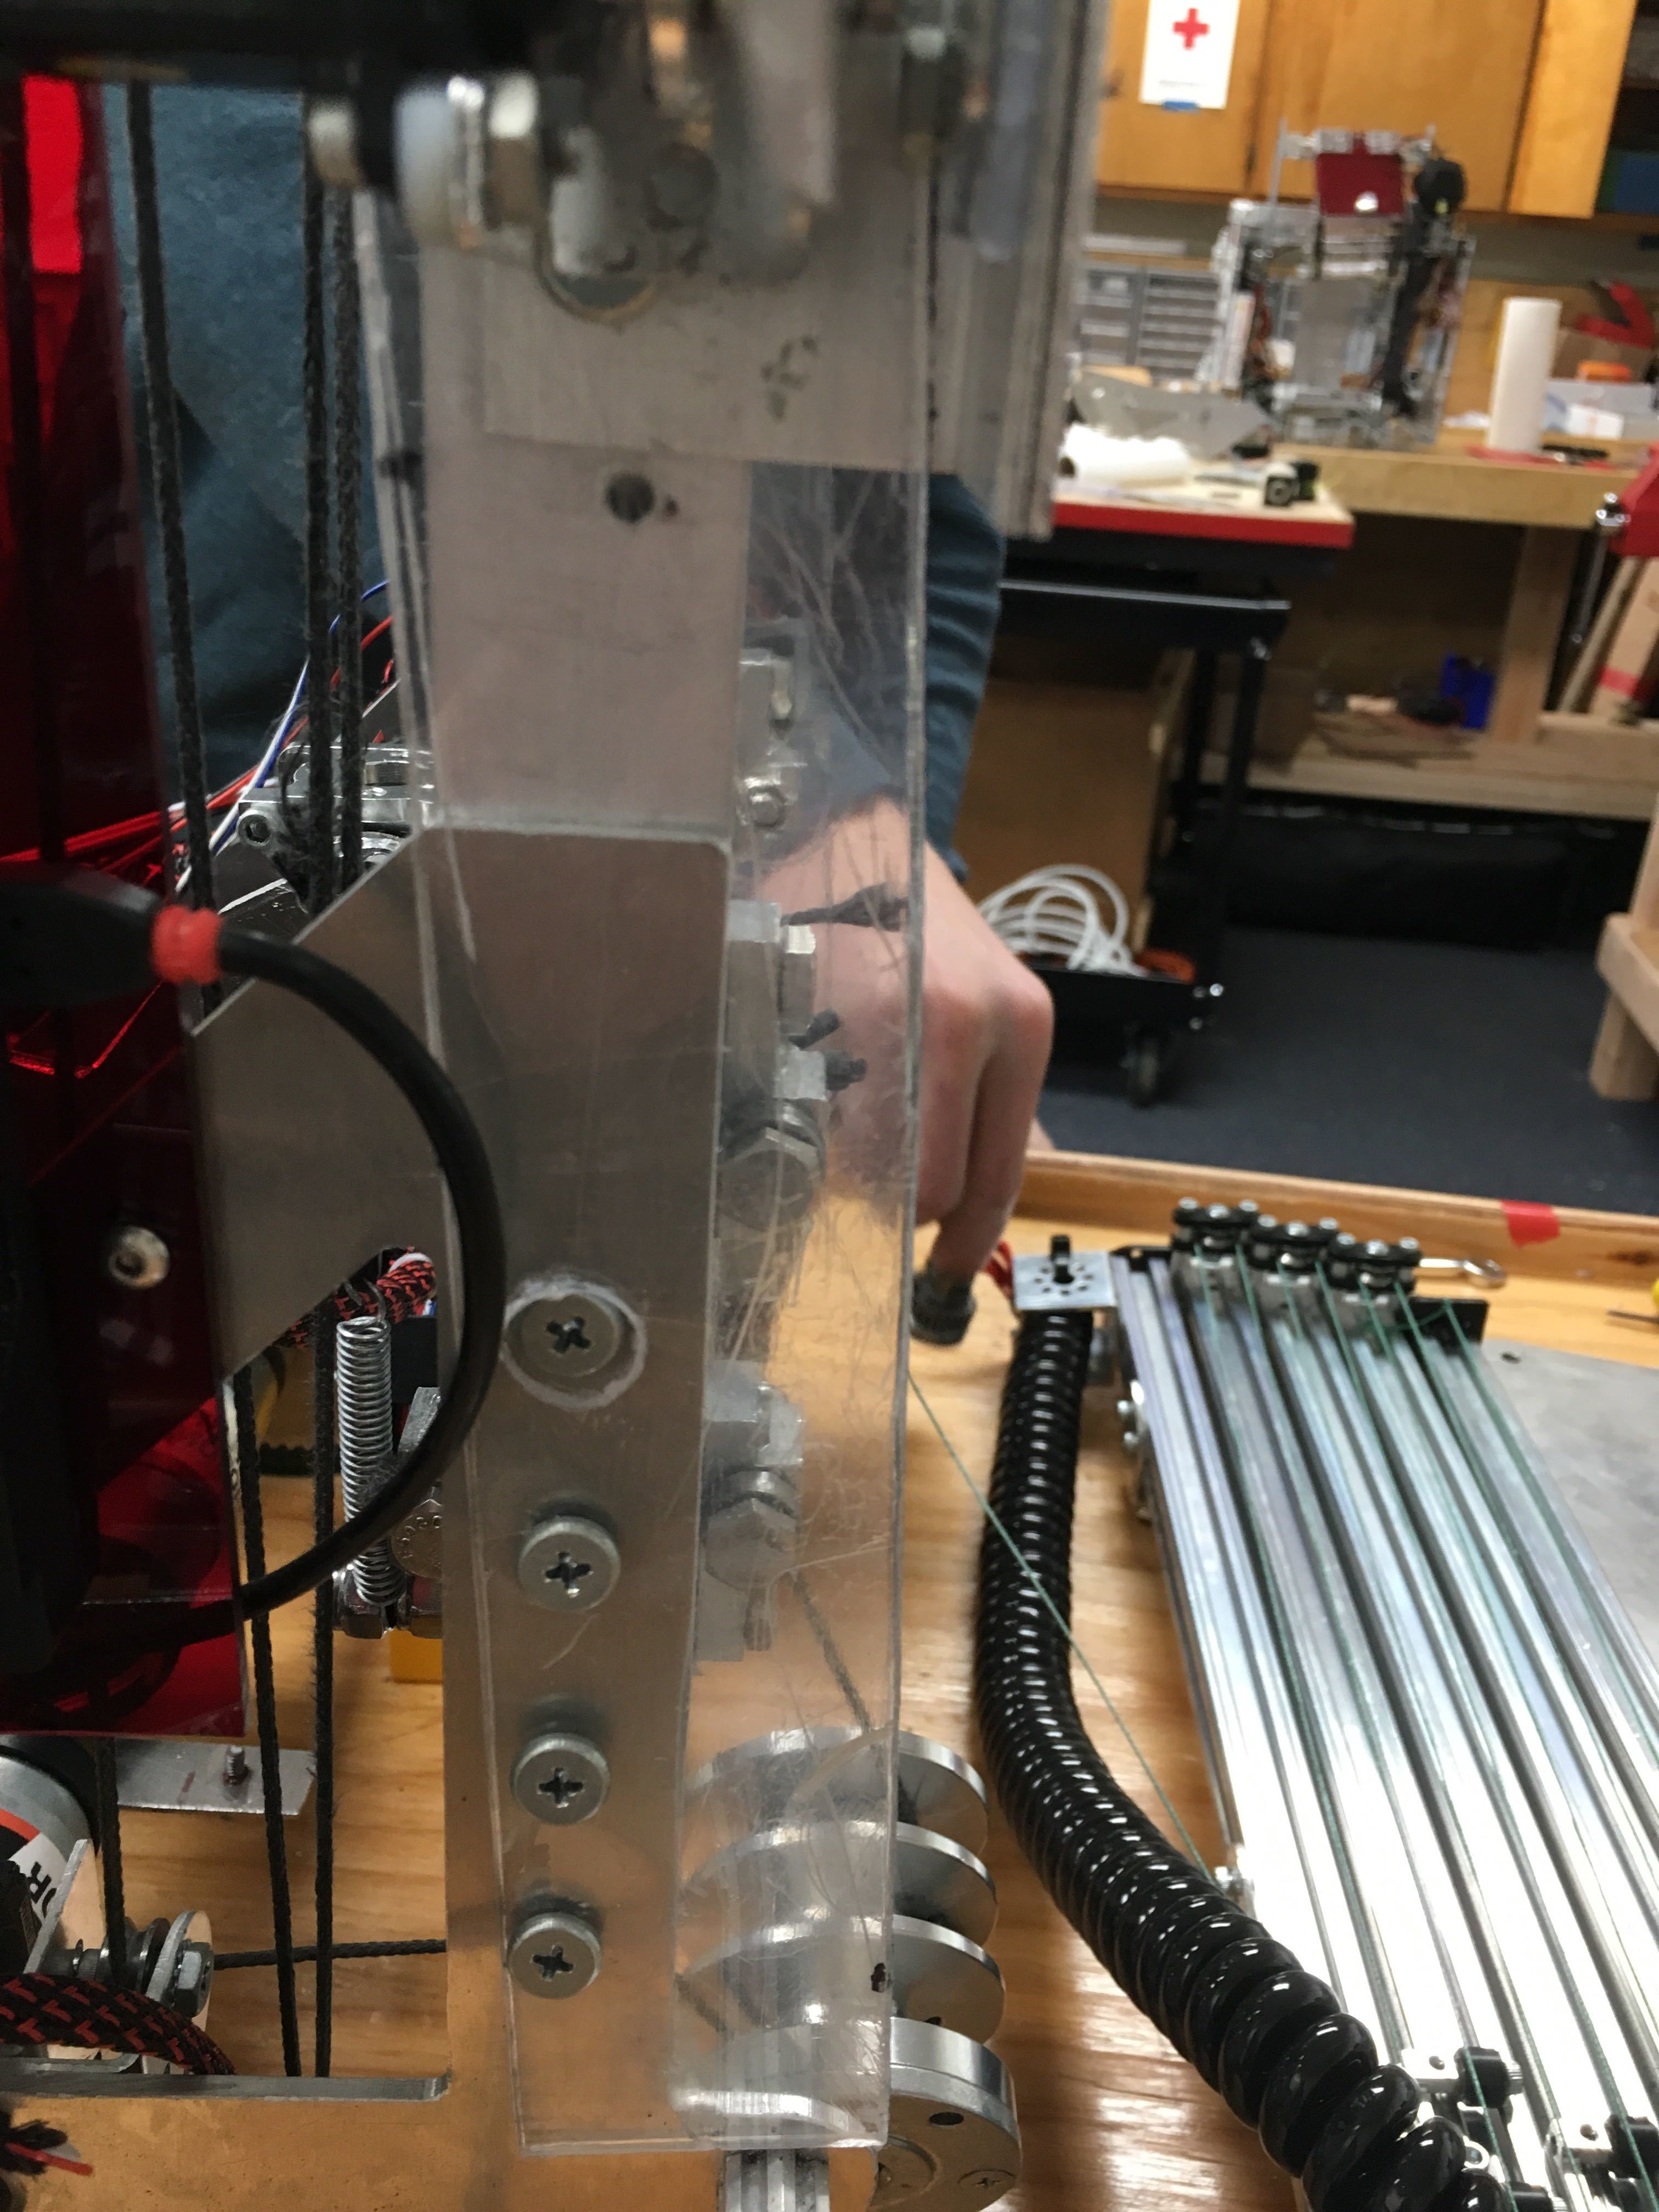
\includegraphics[width=.6 \textwidth]{21_01-21/images/liftskids.JPG}
    \caption{Lift Skids}
    \label{fig:skids}
\end{figure}

\end{document}